\documentclass[lang=en,mode=normal,device=normal,color=blue,12pt]{elegantnote}
\usepackage{amsmath,amssymb}
\usepackage{bbm}
\usepackage{tcolorbox}
\usepackage{graphicx}
\usepackage{booktabs}
 \usepackage{subfigure}
 \usepackage{algorithm}
\usepackage{algpseudocode}
\DeclareMathOperator*{\E}{\mathbb{E}}
\DeclareMathOperator*{\1}{\mathbbm{1}}
\DeclareMathOperator*{\R}{\mathbbm{R}}
\DeclareMathOperator*{\argmax}{arg\,max}
\DeclareMathOperator*{\argmin}{arg\,min}

\title{Note: Proximal Policy Optimization}

\author{Yanqing Wu}
\institute{Viwistar Robotics}

% \version{0.1.0}
\date{\today}

\begin{document}
\maketitle

\newpage

PPO: first-order method, on-policy learning, actor-critic structure

\section{Background}

In normal policy gradient, training can be unstable due to sparse reward and sampled target, causing dramatic changes on the policy; this eventually collapses performance.
To enhance training stability, we want to limit the parameter updates that would change the policy too much at one step.
With this goal, True Region Policy Optimization (TRPO) and Proximal Policy Optimization (PPO) was introduced.
TRPO delimit the KL divergence with a constraint. More specifically, TRPO updates policies by taking the largest step possible to improve performance while satisfying the constraint on how close the new and old policies are allowed to be.
However, TRPO is complicated to implement and is computational-heavy (from the computation of second-order derivative of KL-divergence). PPO simplifies it by using a \textbf{clipped surrogate objective} while retaining similar constraints and similar performance.
Instead of enforcing a hard constraint as in TRPO, PPO formalized the constraint as a penalty in the objective function.

There are two primary variants of PPO: PPO-Penalty and PPO-Clip.

\textbf{PPO-Penalty} approximately solves a KL-constrained update like TRPO, but penalizes the KL-divergence in the objective function instead of making it a hard constraint, and automatically adjusts the penalty coefficient throughout training so that it is scaled appropriately.

\textbf{PPO-Clip} does not have a KL-divergence term in the objective and does not have a constraint at all. Instead relies on specialized clipping in the objective function to remove incentives for the new policy to drift from the old policy, PPO does hard clipping the policy ratio to be within a small range around 1.0, where 1.0 means the new policy is the same as old.

 According to the PPO paper, PPO-Penalty performs worse than PPO-Clip.

\newpage
\section{Implementation}

\subsection{OpenAI PPO}

\begin{figure}[!ht]
  \centering
  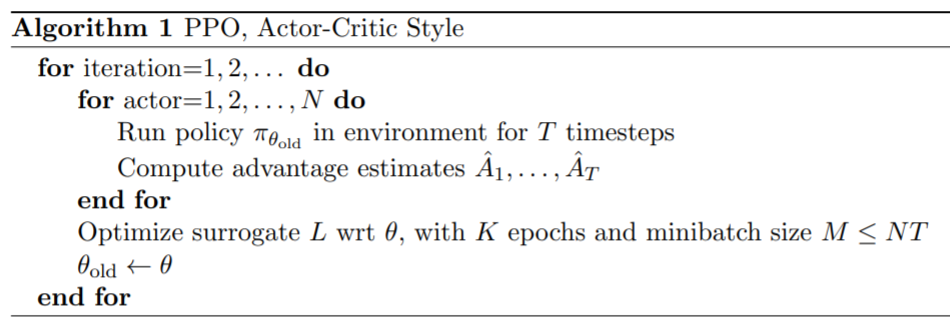
\includegraphics[width=0.7\linewidth]{ppo_openai.PNG}
  \caption{Screenshot of OpenAI PPO algorithm}
  \label{fig:ppo}
\end{figure}

Objective loss is given by
\[
L_t^{CLIP+VF+S}(\theta) = \hat{\E_t} [L_t^{CLIP}(\theta) - c_1 L_t^{VF} + c_2 S[\pi_\theta](s_t)]
\]
where $c_1,c_2$ are coefficients, $\theta$ is a vector of policy parameters, $S$ is entropy bonus, $L^{CLIP}$ is given by
\[
L^{CLIP}(\theta) = \hat{\E_t}[min(r_t(\theta)\hat{A_t},clip(r_t(\theta,1-\epsilon,1+\epsilon)\hat{A_t})]
\]
and squared-error loss $L^{VF}$ is given by
\[
(V_\theta(s_t) - V_t^{target})^2
\]
Truncated version of advantage estimator $\hat{A_t}$ (for policy gradient implementation) is given by
\[
\hat{A_t} = \delta_t + (\gamma \lambda)\delta_{t+1} + \cdots + (\gamma\lambda)^{T-t+1}\delta_{T-1}
\]
where $ \delta_t = r_t + \gamma V(s_{t+1}) - V(s_t) $.
The surrogate loss $L$ is optimized with minibatch Stochastic Gradient Descent (SGD) on $NT$ timesteps of data (where $N$ is the number of parallel actors and $T$ is timesteps).

Another version of $L^{CLIP}$ is as follows:
$$ L(s,a,\theta_k,\theta) = \min\left(
\frac{\pi_{\theta}(a|s)}{\pi_{\theta_k}(a|s)}  A^{\pi_{\theta_k}}(s,a), \;\;
g(\epsilon, A^{\pi_{\theta_k}}(s,a))
\right) $$
where $g(\epsilon,A) = (1+\epsilon)A$ when $A \geq 0$ and $g(\epsilon,A) = (1-\epsilon)A$ when $A < 0$. Through some simplifications, we see that probability ratio $\frac{\pi_{\theta}(a|s)}{\pi_{\theta_k}(a|s)}$ is clipped at $1+\epsilon\;(A>0)$ and $1-\epsilon\;(A<0)$. The hyperparameter $\epsilon$ specifies how much the new policy is allowed to change from the old policy (while still profiting the objective). Therefore, the clipping acts as a regularizer by discouraging the policy to change dramatically.
 
\newpage
\subsection{DeepMind PPO}

DeepMind paper provides a more detailed pseudocode than OpenAI. According to DeepMind pseudo-code of PPO (\ref{fig:ppo})

\begin{figure}[!ht]
  \centering
  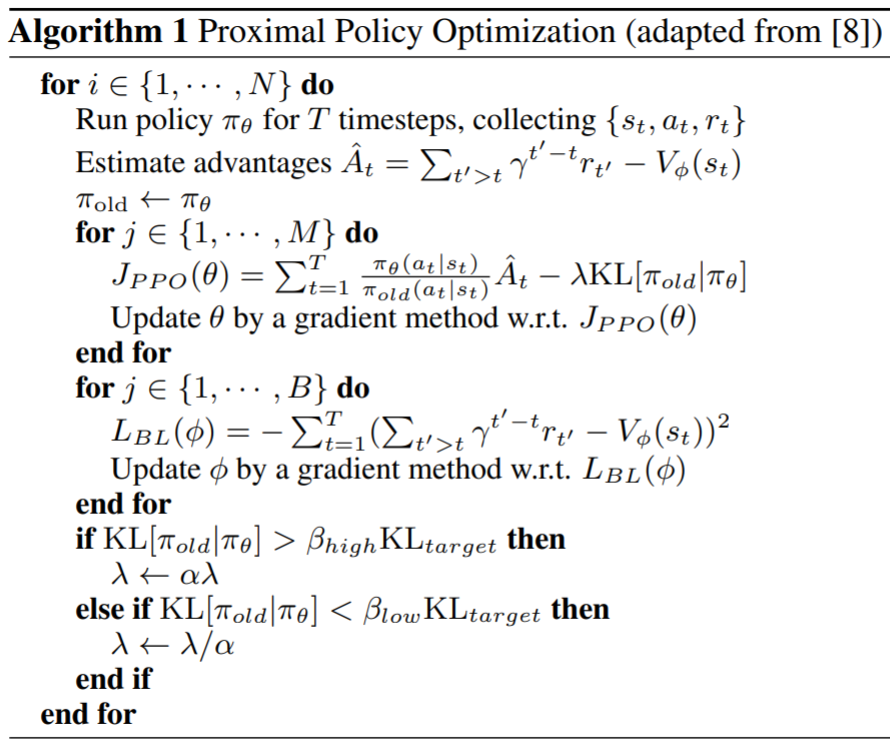
\includegraphics[width=0.7\linewidth]{ppo.PNG}
  \caption{Screenshot of DeepMind PPO algorithm}
  \label{fig:ppo}
\end{figure}

In this algorithm, $KL_{target}$ is the desired change in the policy per iteration.
The Actor maximizes $J_{PPO}$, and Critic minimizes $L_{BL}$.

\section{Reference}
Will update later.


%\bibliography{references.bib}

\end{document}
















